% Created 2021-01-15 Fri 12:46
% Intended LaTeX compiler: pdflatex
\documentclass[11pt]{article}
\usepackage[utf8]{inputenc}
\usepackage[T1]{fontenc}
\usepackage{graphicx}
\usepackage{grffile}
\usepackage{longtable}
\usepackage{wrapfig}
\usepackage{rotating}
\usepackage[normalem]{ulem}
\usepackage{amsmath}
\usepackage{textcomp}
\usepackage{amssymb}
\usepackage{capt-of}
\usepackage{hyperref}
\usepackage{amsthm}
\usepackage{url}
\usepackage[margin=1.25in]{geometry}
\usepackage{hyperref}
\usepackage[dvipsnames]{xcolor}
\usepackage{booktabs}
\usepackage{enumitem}
\newtheorem*{definition}{Definition}
\newtheorem*{example}{Example}
\newtheorem*{theorem}{Theorem}
\newtheorem*{corollary}{Corollary}
\newtheorem*{exercise}{Exercise}
\newtheorem*{problem}{Problem}
\newtheorem{question}{Question}
\newcommand{\gr}{\textcolor{ForestGreen}}
\newcommand{\rd}{\textcolor{red}}
\newcommand{\R}{\mathbb{R}}
\newcommand{\p}{\mathbb{P}}
\newcommand{\frall}{\ \forall}
\author{Chris Ackerman\thanks{I worked on this problem set with Ekaterina Gurkova, Luna Shen, Ben Pirie and Ali Haider Ismail.}}
\date{\today}
\title{Econ202B HW1}
\hypersetup{
 pdfauthor={Chris Ackerman\thanks{I worked on this problem set with Ekaterina Gurkova, Luna Shen, Ben Pirie and Ali Haider Ismail.}},
 pdftitle={Econ202B HW1},
 pdfkeywords={},
 pdfsubject={},
 pdfcreator={Emacs 28.0.50 (Org mode 9.3)}, 
 pdflang={English}}
\begin{document}

\maketitle
\tableofcontents

\newpage

\section{Question 1}
\label{sec:org67d4e06}

  \begin{enumerate}
\item
\begin{enumerate}
\item The worker can only be fired when $s = E$, and can only choose to accept a job when $s = U$. There is no other relevant information for $\{s_t\}$.
\item $ $ \\
\begin{center}
\begin{tabular}[]{ccc}
& E & U \\ \cline{2-3}
E & \multicolumn{1}{|c}{$1 - \delta$} & \multicolumn{1}{|c|}{$\delta$} \\ \cline{2-3}
U & \multicolumn{1}{|c}{$\lambda (1 - F(w^*))$} & \multicolumn{1}{|c|}{$1 - \lambda (1 - F(w^*))$} \\ \cline{2-3}\\
\end{tabular}
\end{center}
\item Using the intuition from the ``lake'' model, we can set up the steady state flows into and out of unemployment as
\begin{align*}
u_{t + 1} &= u_t - u_t (\lambda (1 - F(w^*))) + (1 - u_t) \delta \\
\implies u &= \frac{\delta}{\lambda (1 - F(w^*)) + \delta}
\end{align*}
\item We want to multiply the $UU$ entry in the transition matrix by the $UE$ matrix (1 period of unemployment, then a transition to employment):
\[
(1 - \lambda(1 - F(w^*)))\cdot (\lambda(1 - F(w^*))).
\]
\item Just like in the last answer, we want to multiply the $UU$ entry in the transition matrix but the $UE$ matrix, but this time we need to take the $UU$ entry to the $t$ power to account for the duration of the unemployment spell:
\[
(1 - \lambda(1 - F(w^*)))^t \cdot (\lambda(1 - F(w^*))).
\]
\item 
\[
\sum^\infty_{t = 1} t \cdot (1 - \lambda (1 - F(w^*)))^t \cdot (\lambda (1 - F(w^*)))
\]
\end{enumerate}
\item 
\begin{align*}
w^* &= b + \frac{\lambda}{\delta} \int^{\overline{w}}_{w^*} [1 - F(w)]dw\\
&= b + \frac{\lambda}{\delta}\int^{\overline{w}}_{w^*} \frac{[1 - F(w)]dw}{1 - F(w^*)}\cdot [1 - F(w^*)]\\
&= b + \frac{\lambda}{\delta} (\mathbb{E} [w \mid w \ge w^*] - w^*)[1 - F(w^*)]\\
\delta w^* &= \delta b + \lambda (\mathbb{E}[w \mid w \ge w^*] - w^*)[1 - F(w^*)]\\
w^* (\delta + \lambda[1 - F(w^*)]) &= \delta b + \lambda \mathbb{E}[w \mid w \ge w^*][1 - F(w^*)]\\
\implies w^* &= \frac{\delta}{\delta + \lambda[1 - F(w^*)]} b + \frac{\lambda [1 - F(w^*)]}{\delta + \lambda[1 - F(w^*)]} \mathbb{E}[w \mid w \ge w^*]
\end{align*}
This equation shows that \(w^*\) is the expected return at the stationary distribution. The first term multiplies the probability of being unemployed by the unemployment benefit, and the second term multiplies the probability of being employed by the expected wage. When \(\beta = 1\) but there is still a probability of being fired, \(w^* < \overline{w}\) because the worker doesn't expect their job to last forever. If we also send \(\delta \to 0\), then \(w^* \to \overline{w}\) because, no matter how many periods the worker spends unemployed this is a measure-zero part of their infinite life, and their entire payoff is due to the wage they receive.

\item 
\begin{align*}
w^* &= \rho \mathbb{E} [w \mid w \ge w^*] + \frac{\beta \lambda}{1 - \beta(1 - \delta)} \int^{\overline{w}}_{w^*} [1 - F(w)]dw\\
&= \rho M_m w^* + \frac{\beta \lambda}{1 - \beta(1 - \delta)} \frac{\int^{\overline{w}}_{w^*} [1 - F(w)]dw}{1 - F(w^*)} \cdot [1 - F(w^*)] \\
&= \rho M_m w^* + \frac{\beta \lambda}{1 - \beta(1 - \delta)} (\mathbb{E}[w \mid w \ge w^*] - w^*)\cdot [1 - F(w^*)] \\
&= \rho M_m w^* + \frac{\beta \lambda}{1 - \beta(1 - \delta)} (M_m w^* - w^*)\cdot [1 - F(w^*)] \\
w^*(1 - \rho M_m) &= \frac{\beta}{1 - \beta (1 - \delta)} (M_m - 1) \lambda [1 - F(w^*)] w^*\\
\implies \lambda [1 - F(w^*)] &= \frac{1 - \beta(1 - \delta)}{\beta} \frac{1 - \rho M_m}{M_m - 1}
\end{align*}
Using these parameter values, the average duration of unemployment implied by the McCall model is 36 months, which is \textbf{much} larger than the observed value. We can interpret this as a result of the search technology in the McCall model. In the model, workers must apply to jobs sequentially and cannot apply to jobs while they're employed, so it is very hard to find a new job.
  \end{enumerate}
\newpage

\section{Question 2}
\label{sec:org791f9f5}

  \begin{enumerate}
\item
\begin{align*}
V_u &= \beta (1 - \lambda) V_u + \beta \lambda \int^\infty_0 \max \{V_u, V_e(w)\}dw \\
V_e &= w^{1 - \gamma} + \beta [(1 - \delta)V_e(w) + \delta V_u]
\end{align*}
\item 
\begin{align*}
\intertext{Let}
(1 - \beta)V_u &= (w^*)^{1 - \gamma}\\
(w^*)^{1 - \gamma} &= \frac{\beta \lambda}{1 - \beta (1 - \delta)} \int^\infty_{- \infty} \max(0, w^{1 - \gamma} - (w^*)^{1 - \gamma})dF(w)\\
&= \frac{\beta \lambda}{1 - \beta (1 - \delta)} \int^\infty_{w^*} w^{1 - \gamma} - (w^*)^{1 - \gamma} dF(w)\\
u &= w^{1 - \gamma} - (w^*)^{1 - \gamma}\\
du &= (1 - \gamma) w^{- \gamma} dw \\
v &= - (1 - F(w))\\
dv &= dF(w)\\
\implies (w^*)^{1 - \gamma} &= \frac{\beta \lambda}{1 - \beta (1 - \delta)} \left(\left.(w^{1 - \gamma} - (w^*)^{1 - \gamma})(F(w) - 1)\right|^\infty_{w^*} + \int^\infty_{w^*} (1 - \gamma) w^{- \gamma} (1 - F(w))dw\right)\\
&= \frac{\beta \lambda}{1 - \beta(1 - \delta)} \int^\infty_{w^*} (1 - \gamma)w^{- \gamma} (1 - F(w))dw
\end{align*}
\newpage
\item
$ $\\
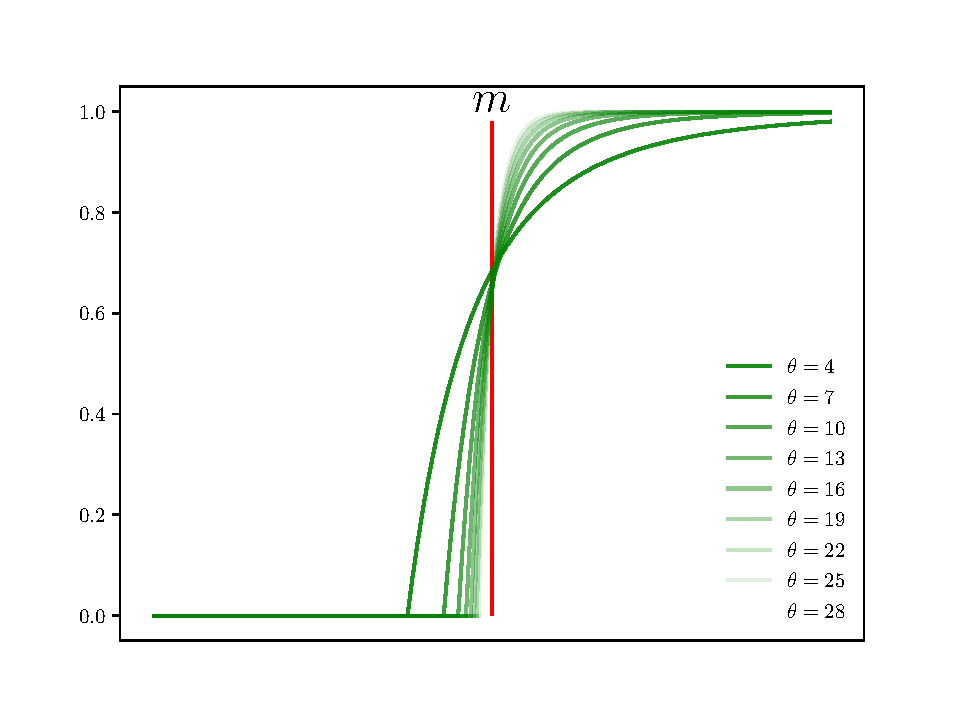
\includegraphics{cdf_graph.pdf}
\item The distribution converges to a point mass on $m$ (the red line in part 3, with flat parts before and after).

\item 
\begin{align*}
w^* &= \frac{\beta}{1 - \beta(1 - \delta)} \int^{\overline{w}}_{w^*} 1 - F(w)dw\\
&= \frac{\beta \lambda}{1 - \beta (1 - \delta)} \int^{\overline{w}}_{w^*} (1 - 1)dw \text{ if } w^* \ge m \\
&= 0 \text{ if } w^* \ge m \Rightarrow\!\Leftarrow \\
w^* &= \frac{\beta \lambda}{1 - \beta (1 - \delta)} \dot (m - w^*) \text{ if } w^* < m \\
w^* &- \frac{\beta \lambda}{1 - \beta(1 - \delta) + \beta \lambda} m
\end{align*}
The reservation wage $w^*$ is below $m$ because the discount factor, probability of getting fired, and probability of drawing an offer (which is less than one) effectively make the worker less patient and more willing to accept any job.

\item
\begin{align*}
w^* &= \frac{\beta \lambda}{1 - \beta(1 - \delta)} \int^{\overline{w}}_{w^*} \left(\frac{w}{\underline{w}}\right)^{- \theta} dw \\
&= \frac{\beta \lambda}{1 - \beta (1 - \delta)} \left(\int^\infty_{\underline{w}}\left(\frac{w}{\underline{w}}\right)^{- \theta} dw + \int^{\overline{w}}_{w^*} 1 - 0 dw\right)\\
\theta &> \frac{\beta \lambda + 1 - \beta (1 - \delta)}{1 - \beta (1 - \delta)}
\end{align*}
$\theta$ must be high enough that there is such a low probability of getting an offer above $\underline{w}$ that the worker is not willing to wait for a job offer from this part of the distribution.
\item
\begin{align*}
w^* &= \frac{\beta \lambda}{1 - \beta (1 - \delta)} \int^\infty_{w^*} \left(\frac{w}{\underline{w}}\right)^{- \theta}dw \\ 
&= \frac{\beta \lambda}{1 - \beta(1 - \delta)} \underline{w}^\theta \frac{1}{\theta - 1} (w^*)^{1 - \theta}\\
w^* &= \left(\frac{\beta \lambda}{1 - \beta(1 - \delta)} \cdot \frac{1}{\theta - 1}\right)^{1 / \theta} \underline{w}
\end{align*}
\item
\begin{align*}
(w^*)^{1 - \gamma} &= \frac{\beta \lambda}{1 - \beta (1 - \delta)} \int^\infty_{w^*} (1 - \gamma) w^{- \gamma} \left(\frac{w}{\underline{w}}\right)^{- \theta} dw \\
&= \frac{\beta \lambda}{1 - \beta (1 - \delta)} \underline{w}^\theta \cdot \frac{1 - \gamma}{\gamma + \theta - 1} (w^*)^{1 - \gamma + \theta}\\
w^* &= \frac{\beta \lambda}{1 - \beta(1 - \delta)} \frac{1 - \gamma}{\gamma + \theta - 1} (w^*)^{1 - \gamma + \theta}\\
w^* &= \left(\frac{\beta \lambda}{1 - \beta (1 - \delta)} \frac{1 - \gamma}{\gamma + \theta - 1}\right)^{1 / \theta} \underline{w}
\end{align*}
\item
We can use the expression from the last section:
\[
w^* = \left(\frac{\beta \lambda}{1 - \beta (1 - \delta)} \rd{\frac{1 - \gamma}{\gamma + \theta - 1}}\right)^{\gr{1 / \theta}} \underline{w}.
\]
When $\theta$ increases, the term in red gets smaller and so does the term in green. The decrease in the red term causes a direct decline in $w^*$; since the term inside brackets is less than one, the decline in the green term indirectly increases $w^*$. Intuitively, we saw earlier in the basic McCall model that drawing from a riskier distribution is better for the worker, since they're throwing out all the low draws anyway, so they don't really care where they come from, and the riskier high draws mean more upside. However, now that we have a risk averse worker, we have to balance these better draws against the worker's natural risk aversion, hence the two terms pushing in opposite directions.
\end{enumerate}
\end{document}